
\section{Architecture Integration}

\subsection{Model Support}

\begin{table}[H]
\centering
\small
\begin{tabular}{llllll}
\toprule
\textbf{Model} & \textbf{Attention class} & \textbf{Nested?} & \textbf{RoPE?} & \textbf{GQA?} & \textbf{Verified} \\
\midrule
DistilBERT & \texttt{MultiHeadSelfAttention} & No & No & No &  \\
RoBERTa & \texttt{BertSelfAttention} (nested) & Yes & No & No &  \\
GPT-2 & \texttt{GPT2Attention} (Conv1D) & No & No & No &  \\
Qwen3.5 & \texttt{Qwen3Attention} & No & Yes & Yes & not tested \\
\bottomrule
\end{tabular}
\end{table}

\subsection{Weight Extraction -- Case by Case}

\subsubsection{DistilBERT (Flat)}

\begin{lstlisting}
extracted["q"] = (src.q\_lin.weight.data, src.q\_lin.bias.data)
extracted["k"] = (src.k\_lin.weight.data, src.k\_lin.bias.data)
extracted["v"] = (src.v\_lin.weight.data, src.v\_lin.bias.data)
extracted["o"] = (src.out\_lin.weight.data, src.out\_lin.bias.data)
\end{lstlisting}

\subsubsection{RoBERTa (Nested)}

Detection:

\begin{lstlisting}
if (hasattr(src, "self") and hasattr(src.self, "query")
    and hasattr(src, "output") and hasattr(src.output, "dense")):
    is\_nested\_encoder = True
elif (cls\_name in ["BertSelfAttention", "RobertaSelfAttention", ...]
      and not has\_out\_lin):
    is\_nested\_encoder = True
\end{lstlisting}

Extraction:

\begin{lstlisting}
s = src.self
extracted["q"] = (s.query.weight.data, s.query.bias.data)
extracted["k"] = (s.key.weight.data, s.key.bias.data)
extracted["v"] = (s.value.weight.data, s.value.bias.data)
# out\_proj is handled by set\_identity -- outer attention.output.dense applies it
\end{lstlisting}

\subsubsection{GPT-2 (Conv1D)}

\begin{lstlisting}
c\_w = src.c\_attn.weight.data.clone()
if "Conv1D" in type(src.c\_attn).\_\_name\_\_:
    c\_w = c\_w.t()
q\_w, k\_w, v\_w = c\_w.chunk(3, dim=0)
extracted["q"] = (q\_w, src.c\_attn.bias.data[:768])
extracted["k"] = (k\_w, src.c\_attn.bias.data[768:1536])
extracted["v"] = (v\_w, src.c\_attn.bias.data[1536:2304])
extracted["o"] = (src.c\_proj.weight.data.t(), src.c\_proj.bias.data)
\end{lstlisting}

\subsubsection{Qwen (GQA + RoPE)}

\begin{lstlisting}
extracted["q"] = (src.q\_proj.weight.data, src.q\_proj.bias.data)
extracted["k"] = (src.k\_proj.weight.data, src.k\_proj.bias.data)
extracted["v"] = (src.v\_proj.weight.data, src.v\_proj.bias.data)
extracted["o"] = (src.o\_proj.weight.data, src.o\_proj.bias.data)
\end{lstlisting}

\subsection{Nested Encoder Handling with `set\_identity`}

RoBERTa and BERT nest attention: \texttt{BertAttention} has both \texttt{self} (Q/K/V) 
and \texttt{output.dense} (output projection). If ASVD applies its own out\_proj 
inside the attention module, and the outer \texttt{attention.output.dense} also 
applies a projection, the result is a \textbf{double projection}.

\textbf{Solution.} For nested encoders, ASVD's out\_proj is set to identity via 
\texttt{set\_identity()}:

\begin{lstlisting}
if proj == "o" and self.is\_nested\_encoder:
    self.out\_proj.set\_identity()
\end{lstlisting}

The identity configuration:

\begin{lstlisting}
def set\_identity(self):
    with torch.no\_grad():
        self.U.data.zero\_()
        self.V.data.zero\_()
        self.S.data.fill\_(1.0)
        r = min(self.rank, self.in\_features, self.out\_features)
        self.U.data[:r, :r].fill\_diagonal\_(1.0)
        self.V.data[:r, :r].fill\_diagonal\_(1.0)
        if self.bias is not None:
            self.bias.data.zero\_()
        self.freeze\_base\_weights()
\end{lstlisting}

Then, in \texttt{forward}:

\begin{lstlisting}
if self.is\_nested\_encoder:
    out = context  # skip out\_proj
else:
    out = self.out\_proj(context)
\end{lstlisting}

\subsection{Injection with Pre-Flight Validation}

The \texttt{inject\_asvd} hook performs a \textbf{pre-flight test}:

\begin{lstlisting}
def inject\_asvd(model=None, layer=None, config=None, ...):
    target\_model = model or ...
    if target\_model is not None:
        return inject\_attention(target\_model, "asvd", ...)
    
    old\_attn = find\_attention(layer)
    target\_config = config or old\_attn.config
    
    if old\_attn is not None:
        try:
            new\_attn = ASVDAttention(target\_config, rank=rank,
                                      pretrained\_attn=old\_attn, **kwargs)
            replace\_attention(layer, new\_attn)
            return new\_attn
        except RuntimeError as err:
            logger.warning(f"Pre-flight weight extraction failed: {err}. Aborting.")
        except Exception as err:
            logger.warning(f"Unexpected error: {err}. Aborting.")
    
    # Fallback to random initialization with warning
    new\_attn = ASVDAttention(target\_config, rank=rank, **kwargs)
    replace\_attention(layer, new\_attn)
    return new\_attn
\end{lstlisting}

\textbf{Key design choice.} ASVD attempts extraction \textbf{first} and aborts 
cleanly on failure. This is safer than NHA/EAT (silent fallback) but 
stricter than A3/AASVD (which log warnings).

\subsection{The `ASVDLinear` Module Structure}

\begin{lstlisting}
class ASVDLinear(nn.Module):
    def \_\_init\_\_(self, in\_features, out\_features, rank,
                 bias=True, lora\_rank=0, freeze\_base=False):
        super().\_\_init\_\_()
        self.U = nn.Parameter(torch.empty(out\_features, rank))
        self.S = nn.Parameter(torch.empty(rank))
        self.V = nn.Parameter(torch.empty(rank, in\_features))
        if bias:
            self.bias = nn.Parameter(torch.empty(out\_features))
        if lora\_rank \textgreater{} 0:
            self.lora\_A = nn.Parameter(torch.empty(lora\_rank, in\_features))
            self.lora\_B = nn.Parameter(torch.zeros(out\_features, lora\_rank))
        self.reset\_parameters()
        if freeze\_base:
            self.freeze\_base\_weights()
\end{lstlisting}

\textbf{Forward pass:}

\begin{lstlisting}
def forward(self, x):
    Vx = F.linear(x, self.V)          # x @ V^T
    SVx = Vx * self.S                  # scale by $\Sigma$
    out = F.linear(SVx, self.U)        # @ U^T
    if self.bias is not None:
        out = out + self.bias
    if self.lora\_rank \textgreater{} 0:
        lora\_out = F.linear(F.linear(x, self.lora\_A), self.lora\_B)
        out = out + lora\_out
    return out * self.output\_scale
\end{lstlisting}

\subsection{Registry}

\begin{lstlisting}
@ATTENTION\_REGISTRY.register("asvd")
@ATTENTION\_REGISTRY.register("asvd\_attention")
class ASVDAttention(BaseAttention):
    ...
\end{lstlisting}

\subsection{Causality}

\textbf{Verification.} Gradient of output at position $i$ w.r.t. input at 
position $j > i$ is zero.

\subsection{Failure Modes}

\begin{table}[H]
\centering
\small
\begin{tabular}{lll}
\toprule
\textbf{Failure} & \textbf{Detection} & \textbf{Response} \\
\midrule
Missing projection & \texttt{copy\_weights} raises & Pre-flight check aborts \\
Small Frobenius norm & Explicit check & Raises RuntimeError \\
Reconstruction error \textgreater{} $\tau$ & Validation & Aborts injection \\
Cross-attention & Explicit check & Raises NotImplementedError \\
\bottomrule
\end{tabular}
\end{table}

\subsection{Cross-Attention Not Supported}

\begin{lstlisting}
if encoder\_hidden\_states is not None:
    raise NotImplementedError("Cross-attention is not supported in ASVDAttention.")
\end{lstlisting}
\begin{lstlisting}

---
\end{lstlisting}

\begin{figure}[H]
\centering
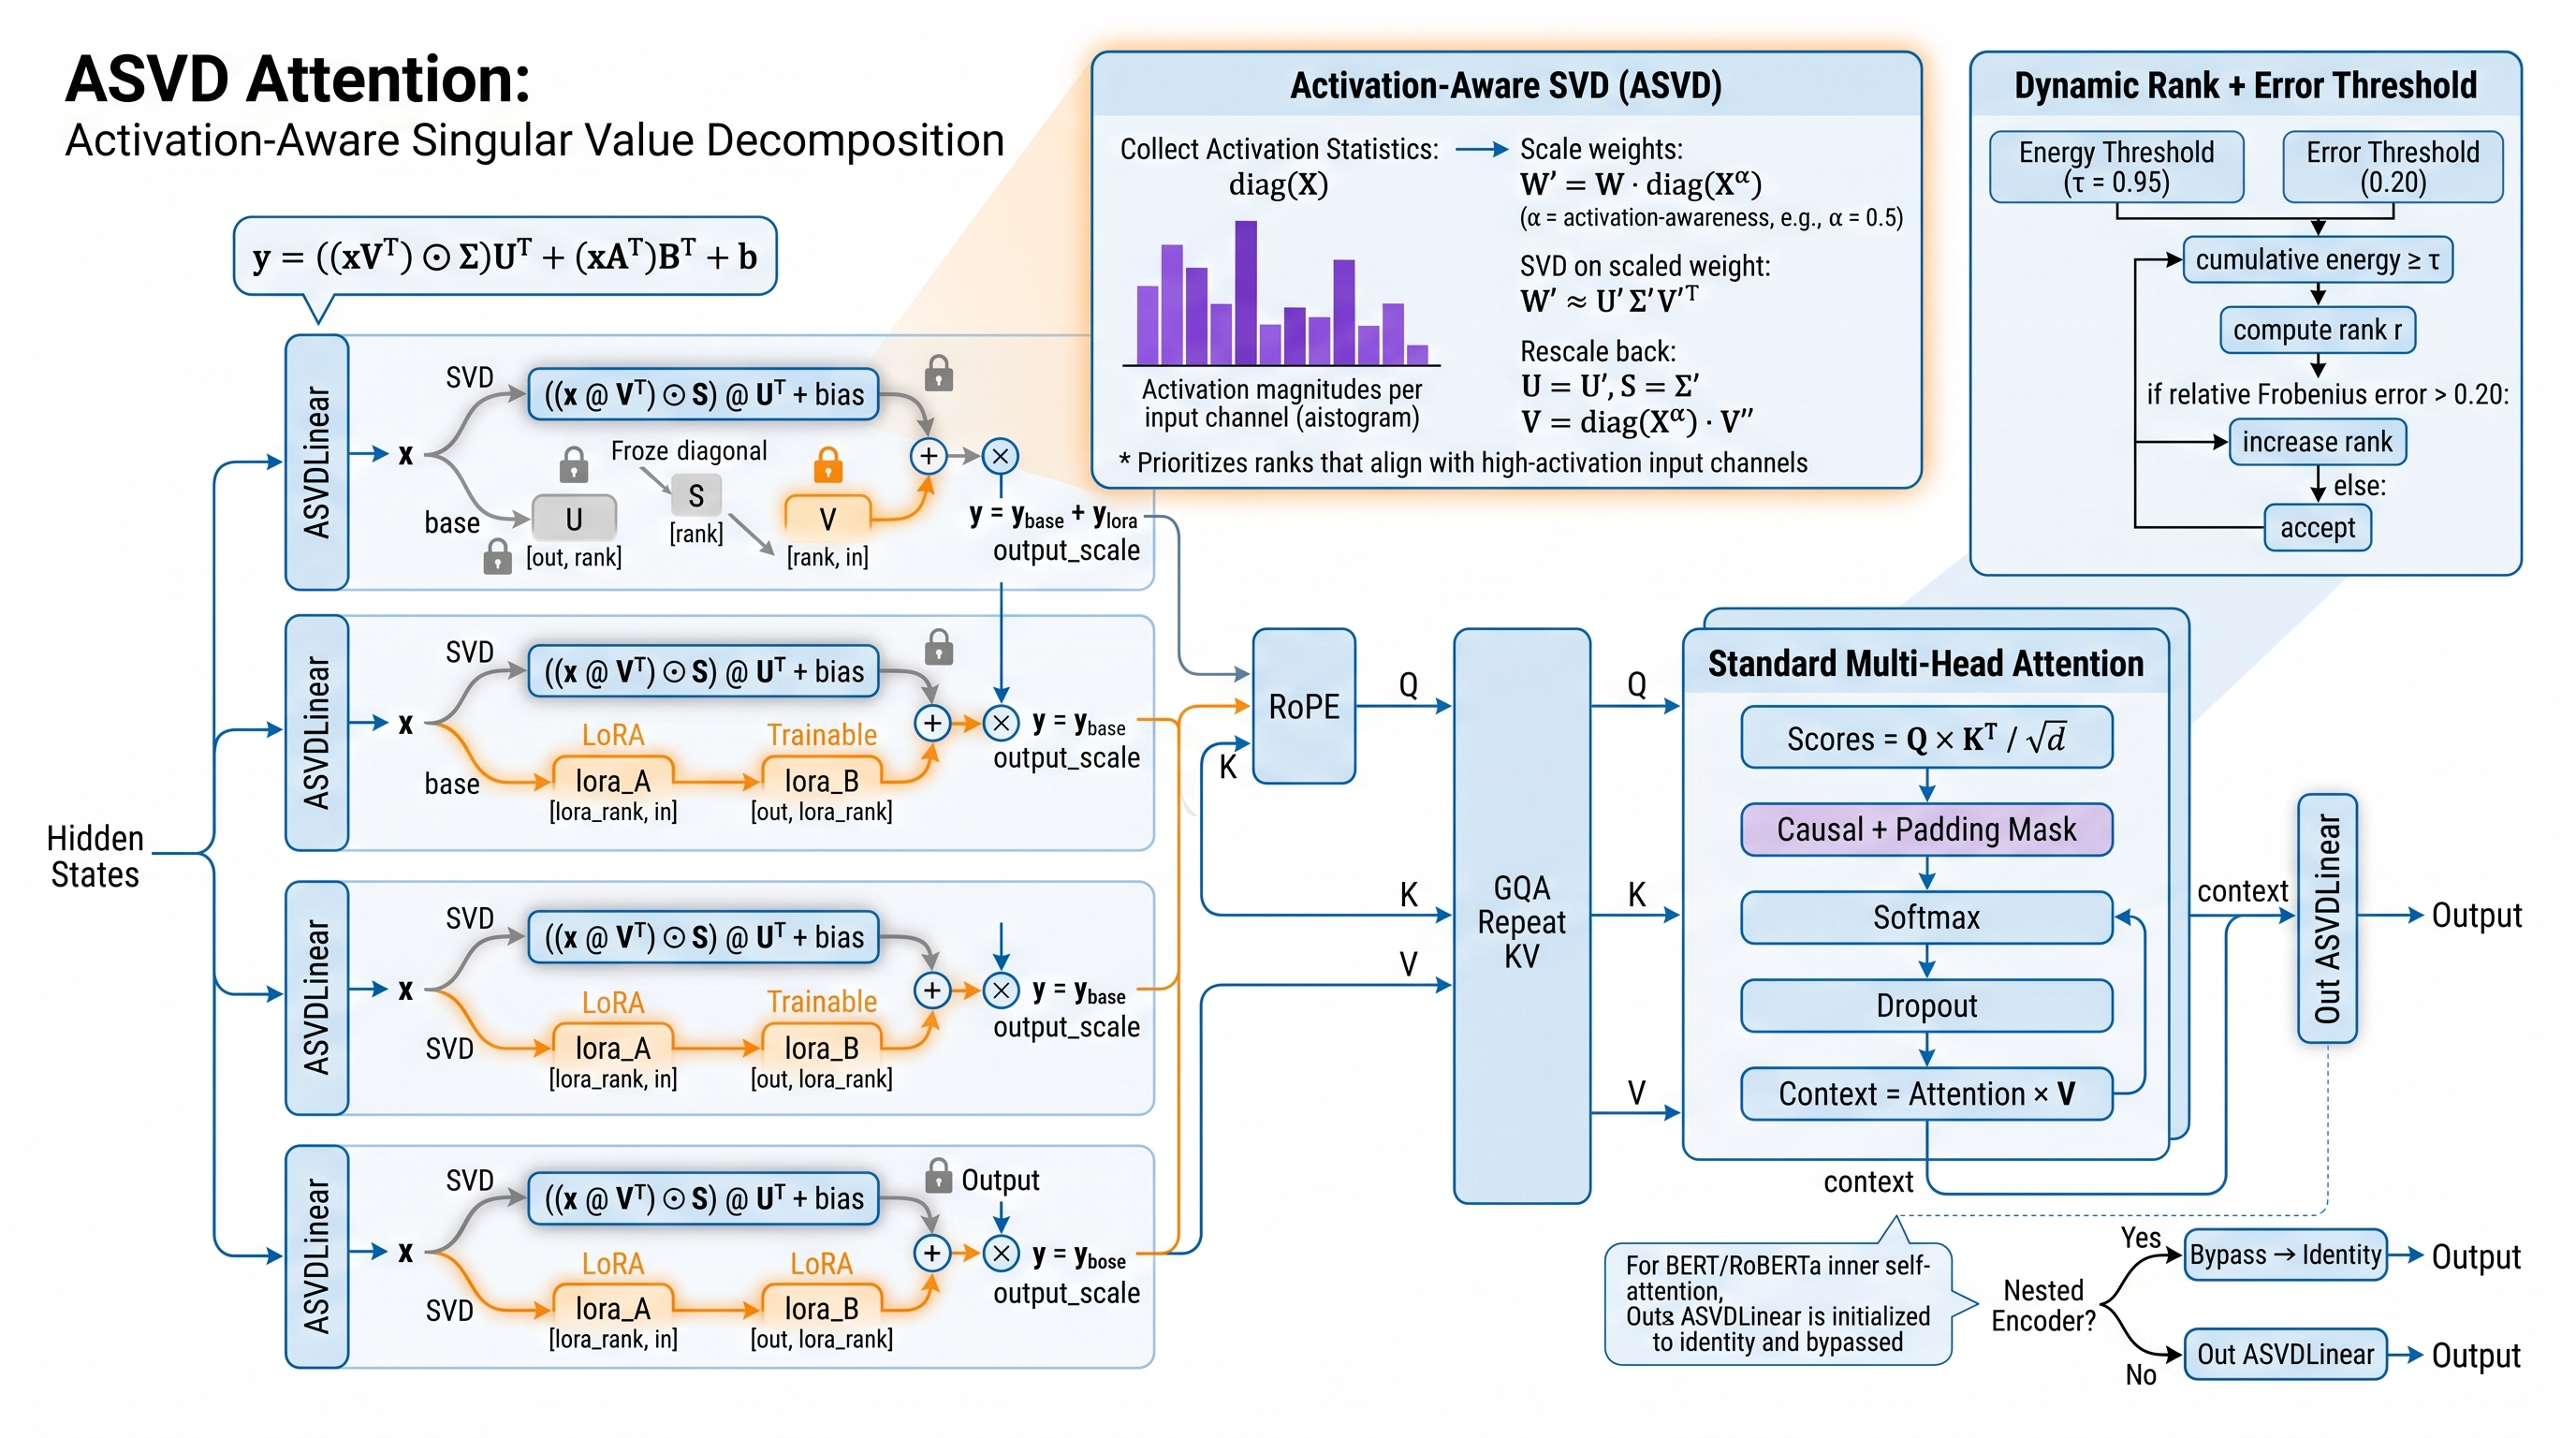
\includegraphics[width=\linewidth]{figures/architecture.jpeg}
\caption{High-level architectural diagram of asvd.}
\label{fig:arch\_asvd}
\end{figure}

